\documentclass{beamer}
\usetheme{Warsaw}

\usefonttheme{professionalfonts}

\usepackage{polski}
\usepackage[utf8]{inputenc}
\usepackage{tabularx}
\usepackage{sourcecodepro}
\usepackage{listings}
\usepackage{color} %use color
\definecolor{mygreen}{rgb}{0,0.6,0}
\definecolor{mygray}{rgb}{0.5,0.5,0.5}
\definecolor{mymauve}{rgb}{0.58,0,0.82}

%Customize a bit the look
\lstset{ %
backgroundcolor=\color{white}, % choose the background color; you must add \usepackage{color} or \usepackage{xcolor}
basicstyle=\tiny, % the size of the fonts that are used for the code
breakatwhitespace=false, % sets if automatic breaks should only happen at whitespace
breaklines=true, % sets automatic line breaking
captionpos=b, % sets the caption-position to bottom
commentstyle=\color{mygreen}, % comment style
deletekeywords={...}, % if you want to delete keywords from the given language
escapeinside={\%*}{*)}, % if you want to add LaTeX within your code
extendedchars=true, % lets you use non-ASCII characters; for 8-bits encodings only, does not work with UTF-8
frame=single, % adds a frame around the code
keepspaces=true, % keeps spaces in text, useful for keeping indentation of code (possibly needs columns=flexible)
keywordstyle=\color{blue}, % keyword style
% language=Octave, % the language of the code
morekeywords={*,...}, % if you want to add more keywords to the set
numbers=left, % where to put the line-numbers; possible values are (none, left, right)
numbersep=5pt, % how far the line-numbers are from the code
numberstyle=\tiny\color{mygray}, % the style that is used for the line-numbers
rulecolor=\color{black}, % if not set, the frame-color may be changed on line-breaks within not-black text (e.g. comments (green here))
showspaces=false, % show spaces everywhere adding particular underscores; it overrides 'showstringspaces'
showstringspaces=false, % underline spaces within strings only
showtabs=false, % show tabs within strings adding particular underscores
stepnumber=1, % the step between two line-numbers. If it's 1, each line will be numbered
stringstyle=\color{mymauve}, % string literal style
tabsize=2, % sets default tabsize to 2 spaces
title=\lstname % show the filename of files included with \lstinputlisting; also try caption instead of title
}
%END of listing package%

\definecolor{darkgray}{rgb}{.4,.4,.4}
\definecolor{purple}{rgb}{0.65, 0.12, 0.82}

%define Javascript language
\lstdefinelanguage{TypeScript}{
keywords={typeof, new, true, false, catch, function, return, catch, switch, var, if, in, while, do, else, case, break, let, const, class, export, import, this, throw, implements},
keywordstyle=\color{blue}\bfseries,
ndkeywords={boolean, number, string, object, any, void, null, undefined},
ndkeywordstyle=\color{darkgray}\bfseries,
identifierstyle=\color{black},
sensitive=false,
comment=[l]{//},
morecomment=[s]{/*}{*/},
commentstyle=\color{purple}\ttfamily,
stringstyle=\color{red}\ttfamily,
morestring=[b]',
morestring=[b]",
morestring=[b]`
}

\lstset{
language=TypeScript,
extendedchars=true,
basicstyle=\tiny\ttfamily,
showstringspaces=false,
showspaces=false,
numbers=left,
numberstyle=\tiny\ttfamily,
numbersep=9pt,
tabsize=2,
breaklines=true,
showtabs=false,
captionpos=b
}

\title{Angular}
\subtitle{Warsztaty}
\author{Piotr Wolny}
\institute{e-point SA}
\date{\today}

\begin{document}

\begin{frame}
    \titlepage
\end{frame}

\begin{frame}
    \frametitle{Wprowadzenie}
    \begin{itemize}
        \item AngularJS od 2010 roku
        \item Angular 2+ od 2016 roku
        \item napisany od nowa w TypeScript
        \item versus Ember
        \item versus React
        \item versus Vue.js
    \end{itemize}
\end{frame}

\begin{frame}[fragile]
    \frametitle{TypeScript}
    \begin{itemize}
        \item nadzbiór JavaScript
        \item opcjonalne typowanie
\begin{lstlisting}
let fullName: string = 'Bob Bobbington';
let age: number = 37;
let sentence: string = `Hello, my name is ${fullName}.

I'll be ${age + 1} years old next month.`;
let array: number[] = [1, 2, 3];
let tuple: [string, number] = ["hello", 10];
enum Color {Red, Green, Blue}
let c: Color = Color.Green;
\end{lstlisting}
        \item specjalne typy: \lstinline{any, void, null, undefined, object}
        \item dekoratory - adnotacje w świecie JS
    \end{itemize}
\end{frame}

\begin{frame}
    \frametitle{Przegląd}
    \begin{itemize}
        \item Moduły
            \begin{itemize}
                \item grupują powiązane ze sobą elementy źródłowe
                \item aplikacja składa się z co najmniej 1 modułu (\lstinline{AppModule})
                \item mogą importować inne moduły
                \item klasa z dekoratorem \lstinline{@NgModule()}
                \item nie mylić z modułami JS
            \end{itemize}
        \item Komponenty
            \begin{itemize}
                \item widoki, z których składa się aplikacja
                \item klasa z dekoratorem \lstinline{@Component()}
                \item szablon HTML i style CSS
            \end{itemize}
        \item Serwisy
            \begin{itemize}
                \item dostarczają funkcje niezwiązane bezpośrednio z warstwą widoku
                \item wstrzykiwanie zależnośaci
                \item klasa z dekoratorem \lstinline{@Injectable()}
            \end{itemize}
    \end{itemize}
\end{frame}

\begin{frame}
    \frametitle{Przegląd}
    \begin{center}
	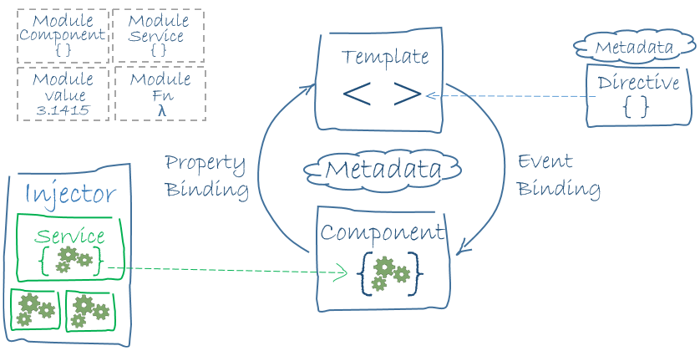
\includegraphics[scale=0.4]{overview2.png}
    \end{center}
\end{frame}

\begin{frame}
    \frametitle{Angular CLI}
    \begin{itemize}
        \item \lstinline{ng version} (7.1.0!)
        \item \lstinline{ng new}
        \item \lstinline{ng build --prod}
        \item \lstinline{ng serve}
        \item \lstinline{ng test}
        \item \lstinline{ng lint}
        \item \lstinline{ng generate}
    \end{itemize}
\end{frame}

\begin{frame}
    \frametitle{Ćwiczenie 1: Angular CLI}
    \begin{itemize}
        \item Wygenerować nowy projekt ng-workshop (scss, ruting)
        \item Uruchomić aplikację
        \item Sprawdzić, czy działa pod adresem http://localhost:4200
        \item Uruchomić testy
        \item Uruchomić sprawdzanie stylu (\lstinline{ng lint})
        \item Zintegrować sprawdzanie stylu z IntelliJ IDEA
        \item Usunąć wygenerowaną zawartość szablonu (\lstinline{app.component.html})
        \item Wygenerować nowy komponent (header) z napisem "ng-workshop"
        \item Sprawdzić, czy aplikacja odświeżyła się automatycznie
    \end{itemize}
\end{frame}

\begin{frame}
    \frametitle{Struktura aplikacji}
    Najważniejsze katalogi i pliki.
    \begin{itemize}
        \item \lstinline{package.json}
        \item \lstinline{angular.json}
        \item \lstinline{src/index.html}
        \item \lstinline{src/styles.scss}
        \item \lstinline{src/app/app.module.ts}
        \item \lstinline{src/app/app.component.ts}
    \end{itemize}
\end{frame}

\begin{frame}
    \frametitle{Ruting i nawigacja - podstawy}
    \begin{itemize}
        \item Moduł \lstinline{RouterModule} (@angular/router)
        \item Dyrektywa \lstinline{<router-outlet>}
        \item Dyrektywa \lstinline{<a routerLink="/jobs">Jobs</a>}
        \item Serwis \lstinline{Router} do nawigacji z kodu źródłowego: \lstinline{router.navigate(ByUrl)}
    \end{itemize}
\end{frame}

\begin{frame}[fragile]
    \frametitle{Ruting - konfiguracja}
\begin{lstlisting}
const routes: Routes = [
  { path: '', component: HomepageComponent },
  { path: 'jobs', component: JobListComponent },
  { path: 'candidates', component: CandidateListComponent },
  { path: '**', component: PageNotFoundComponent },
];

@NgModule({
  imports: [RouterModule.forRoot(routes)],
  exports: [RouterModule]
})
export class AppRoutingModule { }
\end{lstlisting}
\end{frame}

\begin{frame}
    \frametitle{Ćwiczenie 2: Ruting}
    \begin{itemize}
        \item Wygenerować komponenty/strony:
	    \begin{itemize}
                \item \lstinline{homepage}
                \item \lstinline{job-list}
                \item \lstinline{candidate-list}
                \item \lstinline{page-not-found}
	    \end{itemize}
        \item Skonfigurować ruting: \lstinline{/}, \lstinline{/jobs}, \lstinline{/candidates} i \lstinline{/**}
        \item Dodać linki do nagłówka
    \end{itemize}
\end{frame}

\begin{frame}[fragile]
    \frametitle{Komponenty - definicja}
\begin{lstlisting}
@Component({
  selector:    'app-example',
  templateUrl: './example.component.html',
  styleUrls:   ['./example.component.scss']
  providers:   [ ExampleService ]
})
export class ExampleComponent implements OnInit {
/* . . . */
}
\end{lstlisting}
\end{frame}

\begin{frame}[fragile]
    \frametitle{Komponenty - szablon}
\begin{lstlisting}
<h2>Hero List</h2>

<p><i>Pick a hero from the list</i></p>
<ul>
  <li *ngFor="let hero of heroes" (click)="selectHero(hero)">
    {{hero.name}}
  </li>
</ul>

<app-hero-detail *ngIf="selectedHero" [hero]="selectedHero"></app-hero-detail>
\end{lstlisting}
\end{frame}

\begin{frame}
    \frametitle{Komponenty - drzewo}
    \begin{center}
	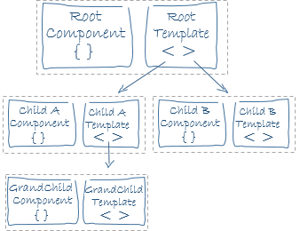
\includegraphics[scale=0.4]{component-tree.png}
    \end{center}
\end{frame}

\begin{frame}
    \frametitle{Komponenty - data binding}
    \begin{center}
	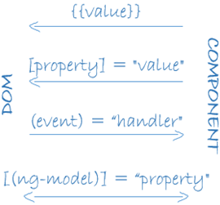
\includegraphics[scale=0.4]{databinding.png}
    \end{center}
\end{frame}

\begin{frame}
    \frametitle{Komponenty - data binding}
    \tiny
    \begin{tabularx}{\textwidth}{X | X | X}
    Kierunek łączenia & Składnia & Typ \\
    \hline \hline
    Jednokierunkowe ze źródła danych do widoku &
    \{\{expression\}\}\newline
    [target]="expression"\newline
    bind-target="expression" &
    Interpolation\newline
    Property\newline
    Attribute\newline
    Class\newline
    Style \\
    \hline
    Jednokierunkowe z widoku do źródła danych &
    (target)="statement"\newline
    on-target="statement" &
    Event \\
    \hline
    Two-way &
    [(target)]="expression"\newline
    bindon-target="expression" &
    Two-way \\
\end{tabularx}
\end{frame}

\begin{frame}
    \frametitle{Komponenty - uproszczony cykl życia}
\tiny
\begin{tabularx}{\textwidth}{l | X | X}
    Metoda & Przeznaczenie & Wykonanie \\
    \hline \hline
    ngOnChanges() & Orzymuje obiekt SimpleChanges, zawierający aktualne i poprzednie wartości właściwości wejściowych. & Wywoływane przed ngOnInit() i przy każdej zmianie właściwości wejściowych (input properties).\\
    \hline
    ngOnInit() & Do inicjalizacji komponentu po ustawieniu właściwości wejściowych (input properties). & Wywoływane raz, po pierwszym ngOnChanges().\\
    \hline
    ngDoCheck() & Do wykrywania zmian, których Angular nie obsłuży automatycznie. & Wywoływane przy każdym przebiegu wykrywania zmian, zaraz po ngOnChanges() i ngOnInit().\\
    \hline
    ngAfterViewInit() & Do działań po inicjalizacji widoku i widoków dzieci. & Wywoływane raz, po pierwszym ngAfterContentChecked().\\
    \hline
    ngOnDestroy() & Do sprzątania przed zniszczeniem komponentu. Należy odsubskrybować Observable i odłączyć handlery zdarzeń. & Wywoływane przed zniszczeniem komponentu.\\
\end{tabularx}
\end{frame}

\begin{frame}[fragile]
    \frametitle{Dyrektywy}
    \begin{itemize}
        \item Klasy z dekoratorem \lstinline{@Directive()}
        \item Komponenty są dyrektywami - \lstinline{@Component()} rozszerza \lstinline{@Directive()}
        \item Dyrektywy strukturalne - dodają, usuwają lub zastępują elementy drzewa DOM, np.: \lstinline{*ngFor}, \lstinline{*ngIf}
\begin{lstlisting}
<div *ngFor="let hero of heroes; let i=index">{{i + 1}} - {{hero.name}}</div>
<app-hero-detail *ngIf="selectedHero"></app-hero-detail>
<div [ngSwitch]="currentHero.emotion">
  <app-happy-hero    *ngSwitchCase="'happy'"    [hero]="currentHero"></app-happy-hero>
  <app-sad-hero      *ngSwitchCase="'sad'"      [hero]="currentHero"></app-sad-hero>
  <app-unknown-hero  *ngSwitchDefault           [hero]="currentHero"></app-unknown-hero>
</div>
\end{lstlisting}
        \item Dyrektywy atrybutów - wpływają na wygląd lub zachowanie istniejących elementów
\begin{lstlisting}
<input [(ngModel)]="hero.name" [ngClass]="currentClasses" [ngStyle]="currentStyles">
\end{lstlisting}
    \end{itemize}
\end{frame}

\begin{frame}
    \frametitle{Ćwiczenie 3: Wyświetlanie danych}
    \begin{itemize}
        \item Dodać klasę \lstinline{Job} z polami \lstinline{code}, \lstinline{name}, \lstinline{description}, \lstinline{validFrom} typu \lstinline{string}
        \item Dodać tablicę \lstinline{jobs: Job[]} do komponentu \lstinline{job-list}
        \item Wyświetlić listę używająć dyrektywy \lstinline{*ngFor}
    \end{itemize}
\end{frame}

\begin{frame}[fragile]
    \frametitle{Serwisy - definicja}
\begin{lstlisting}
@Injectable({ providedIn: 'root' })
export class ExampleService {
/* . . . */
}
\end{lstlisting}
\end{frame}

\begin{frame}
    \frametitle{Wstrzykiwanie zalezności}
    Hierarchiczny system injectorów. Konfiguracja providerów:
    \begin{itemize}
        \item \lstinline|@Injectable(\{ providedIn: 'root' \})|
        \item \lstinline|@NgModule(\{ providers: [\{ provide: LocationStrategy, useClass: HashLocationStrategy \}] \})|
        \item \lstinline|@Component(\{ providers: [ ExampleService ]\})|
    \end{itemize}
    Provider jest instrukcją dla systemu DI, w jaki sposób uzyskać wartość zależności.
\end{frame}

\begin{frame}
    \frametitle{Ćwiczenie 4: Pobieranie danych z serwisu}
    \begin{itemize}
        \item Dodać serwis \lstinline{JobService} zwracający tablicę \lstinline{Job[]}
        \item Dodać zależność od serwisu do komponentu \lstinline{JobListComponent}
        \item Wypełnić tablicę \lstinline{jobs: Job[]} danymi z serwisu
    \end{itemize}
\end{frame}

\begin{frame}
    \frametitle{Pipes}
    \begin{itemize}
        \item Funkcje transformujące dane do wyświetlenia
        \item Klasa z dekoratorem \lstinline{@Pipe()}
        \item Wbudowane: \lstinline{DatePipe}, \lstinline{UpperCasePipe}, \lstinline{LowerCasePipe}, \lstinline{PercentPipe} i inne
        \item Używamy w szablonach: \lstinline!<p>Today is \{\{ today | date \}\}</p>!
        \item Można parametryzować: \lstinline!<p>Today is \{\{ today | date:"MM/dd/yy" \}\}</p>!
        \item Można łączyć w ciągi: \lstinline!<p>Today is \{\{ today | date | uppercase \}\}</p>!
        \item Czyste i nieczyste rury (\textit{pure nad impure pipes})
    \end{itemize}
\end{frame}

\begin{frame}[fragile]
    \frametitle{Pipes - przykład definicji}
    \begin{lstlisting}
@Pipe({name: 'exponentialStrength'})
export class ExponentialStrengthPipe implements PipeTransform {

  transform(value: number, exponent: string): number {
    let exp = parseFloat(exponent);
    return Math.pow(value, isNaN(exp) ? 1 : exp);
  }
}
    \end{lstlisting}
\end{frame}

\begin{frame}
    \frametitle{Ćwiczenie 5: Używanie rur}
    \begin{itemize}
        \item Użyć \lstinline{UppercasePipe} przy wyświetlaniu kodu
        \item Użyć \lstinline{DatePipe} przy wyświetlaniu daty
        \item Napisać własne \lstinline{FormatDatePipe} rozszerzające \lstinline{DatePipe} zakładające specyficzny format
            wyświetlania daty, np.: MM/dd/yy
    \end{itemize}
\end{frame}

\begin{frame}[fragile]
    \frametitle{Komunikacja z API HTTP}
    \lstinline{HttpClient} z modułu \lstinline{HttpClientModule} (@angular/common/http)
    \begin{itemize}
        \item Używamy w serwisach:
\begin{lstlisting}
export class ExampleService {
  constructor(private http: HttpClient) { }
}
\end{lstlisting}
        \item Typujemy odpowiedź: \lstinline{this.http.get<DataType>(url)}
        \item Zwraca \lstinline{Observable<DataType>}
        \item \lstinline{this.http.post<DataType>(url, data)}
    \end{itemize}
\end{frame}

\begin{frame}[fragile]
    \frametitle{RxJS - Observables}
    \begin{itemize}
        \item Asynchoniczny strumień wartości.
        \item Pozwalają na wymianę komunikatów pomiędzy nadawcą a potencjalnie wieloma subskrybentami.
        \item Promise dostarcza tylko jedną wartość.
        \item Promise jest gorliwy, Observable leniwe - jeśli nikt nie subskrybuje, nic się nie dzieje.
        \item Subskrypcja:
\begin{lstlisting}
myObservable.subscribe(
  x => console.log('Observer got a next value: ' + x),
  err => console.error('Observer got an error: ' + err),
  () => console.log('Observer got a complete notification')
);
\end{lstlisting}
        \item Przetwarzanie wartości:
\begin{lstlisting}
const squareOdd = of(1, 2, 3, 4, 5)
  .pipe(
    filter(n => n % 2 !== 0),
    map(n => n * n)
  );
\end{lstlisting}
    \end{itemize}
\end{frame}

\begin{frame}[fragile]
    \frametitle{Proxy do backendu}
    Ze względu na reguły CORS nie możemy wykonywać bezpośrednio żądań do API na innej domenie / innym porcie.
    Możemy skonfigurować lokalne proxy do API dodając plik src/proxy.conf.json:
\begin{lstlisting}
{
  "/api": {
    "target": "http://ng-workshop-api.herokuapp.com",
    "secure": false,
    "pathRewrite": {
      "^/api": ""
    },
    "changeOrigin": true
  }
}
\end{lstlisting}
    I zmodyfikować angular.json:
\begin{lstlisting}
-            "browserTarget": "ng-workshop:build"
+            "browserTarget": "ng-workshop:build",
+            "proxyConfig": "src/proxy.conf.json"
\end{lstlisting}

\end{frame}

\begin{frame}
    \frametitle{Ćwiczenie 6: Pobieranie danych z API}
    \begin{itemize}
        \item Zaimportować moduł \lstinline{HttpClientModule} w \lstinline{AppModule}
        \item Dodać zależność od \lstinline{HttpClient} w \lstinline{JobService}
        \item Skonfigurować proxy do API
        \item Pobrać dane z API (zwrócić uwagę na format JSON-a z API!)
    \end{itemize}
\end{frame}

\begin{frame}
    \frametitle{PrimeNG}
    \begin{itemize}
        \item Biblioteki gotowych komponentów: Angular Material, PrimeNG, inne
        \item PrimeNG - ponad 80 gotowych komponentów
        \item PrimeIcons - biblioteka z ikonkami
        \item Licencja MIT
        \item Tematy - możliwość zakupu gotowych "ubrań"
        \item https://www.primefaces.org/primeng/
    \end{itemize}
\end{frame}

\begin{frame}[fragile]
    \frametitle{PrimeNG - konfiguracja}
    Dodajemy zależności:
\begin{lstlisting}
npm install primeng --save
npm install primeicons --save
\end{lstlisting}
    Modyfikujemy angular.json:
\begin{lstlisting}
"styles": [
  "node_modules/primeicons/primeicons.css",
  "node_modules/primeng/resources/themes/nova-light/theme.css",
  "node_modules/primeng/resources/primeng.min.css",
  //...
],
\end{lstlisting}
\end{frame}

\begin{frame}
    \frametitle{Ćwiczenie 7: Użycie PrimeNG}
    \begin{itemize}
        \item Skonfigurować PrimeNG w projekcie
        \item Zaimportować moduły MenubarModule i TableModule
        \item Zapoznać się z dokumentacją komponentów Menubar i Table
        \item Użyć ww. komponentów w interfejsie
    \end{itemize}
\end{frame}

\begin{frame}[fragile]
    \frametitle{Reaktywne formularze}
    \begin{itemize}
        \item Dostarczają możliwość definiowania formularzy przez model w kodzie
        \item Definiowane przez model w komponencie: \lstinline{FormControl} i \lstinline{FormGroup}.
        \item \lstinline{FormBuilder} do uproszczenia zapisu.
\begin{lstlisting}
  profileForm = this.fb.group({
    firstName: [''],
    lastName: [''],
    address: this.fb.group({
      street: [''],
      city: [''],
      state: [''],
      zip: ['']
    }),
  });
  constructor(private fb: FormBuilder) { }
\end{lstlisting}
    \end{itemize}
\end{frame}

\begin{frame}[fragile]
    \frametitle{Ruting - zagnieżdżanie}
\begin{lstlisting}
const routes: Routes = [
  { path: '', component: HomepageComponent },
  { path: 'jobs', children: [
    { path: '', component: JobListComponent },
    { path: 'add', component: JobAddComponent },
  ]},
  { path: 'candidates', component: CandidateListComponent },
  { path: '**', component: PageNotFoundComponent },
];
\end{lstlisting}
\end{frame}

\begin{frame}
    \frametitle{Ćwiczenie 8: Użycie formularza do dodawania elementów}
    \begin{itemize}
        \item Zaimportować moduł \lstinline{ReactiveFormsModule} w \lstinline{AppModule}
        \item Dodać nowy komponent \lstinline{add-job}
        \item Skonfigurować zagnieżdżony ruting do nowego komponentu
        \item Zdefiniować formularz w nowym komponencie
        \item Wysłać dane z formularza do API przez serwis
        \item Po udanym zapisaniu wrócić na ekran listy
        \item Używamy komponentów z PrimeNG!
    \end{itemize}
\end{frame}

\begin{frame}[fragile]
    \frametitle{Walidacja}
    \begin{itemize}
        \item Można dodawać funkcje walidacyjne do pól formularza
        \item Walidatory synchroniczne i asynchroniczne
        \item Walidatory wbudowane: min, max, required, requiredTrue, email, minLength, maxLenght, pattern, nullValidator, compose, composeAsync
        \item Klasy CSS: .ng-valid, .ng-invalid, .ng-pending, .ng-pristine, .ng-dirty, .ng-untouched, .ng-touched
        \item Przykład:
\begin{lstlisting}
  addForm = this.formBuilder.group({
    code: ['', [Validators.required, Validators.minLength(3)]],
    name: ['', [Validators.required, Validators.minLength(5)]],
    description: [''],
    validFrom: ['', [Validators.required]]
  });
\end{lstlisting}
        \item \lstinline{FormControl.hasError} - sprawdzanie, czy wystąpił błąd
    \end{itemize}
\end{frame}

\begin{frame}
    \frametitle{Walidacja - HTML}
    TODO: uzupełnić slajd
\end{frame}

\begin{frame}
    \frametitle{Ćwiczenie 9: Walidacja formularza}
    \begin{itemize}
        \item Dodać walidator required do pól: code, name, validFrom
        \item Dodać walidator minLength do pól: code, name
        \item Dodać wyświetlanie walidacji na formularzu używając komponentu message z PrimeNG
    \end{itemize}
\end{frame}

\begin{frame}[fragile]
    \frametitle{Własny walidator}
    \begin{itemize}
        \item Przykład
\begin{lstlisting}
export function forbiddenNameValidator(nameRe: RegExp): ValidatorFn {
  return (control: AbstractControl): {[key: string]: any} | null => {
    const forbidden = nameRe.test(control.value);
    return forbidden ? {'forbiddenName': {value: control.value}} : null;
  };
}
\end{lstlisting}
        \item asynchroniczny: \lstinline{AsyncValidatorFn}
    \end{itemize}
\end{frame}

\begin{frame}
    \frametitle{Ćwiczenie 10: Własny walidator asynchroniczny}
    \begin{itemize}
        \item Dodać walidator sprawdzający przez zapytanie do API, czy kod jest unikalny
        \item Zapewnić, że walidator nie uruchomi się częściej niż raz na 500ms
    \end{itemize}
\end{frame}

\begin{frame}[fragile]
    \frametitle{Ruting z parametrem}
    \begin{itemize}
        \item Przykład
\begin{lstlisting}
const routes: Routes = [
  { path: '', component: HomepageComponent },
  { path: 'jobs', children: [
    { path: '', component: JobListComponent },
    { path: 'add', component: JobAddComponent },
    { path: ':id', component: JobDetailsComponent },
  ]},
  { path: 'candidates', component: CandidateListComponent },
  { path: '**', component: PageNotFoundComponent },
];
\end{lstlisting}
        \item Wyciąganie wartości parametru przez serwis \lstinline{ActivatedRoute}, właściwość \lstinline{paramMap}
    \end{itemize}
\end{frame}

\begin{frame}
    \frametitle{Ćwiczenie 11: Ekran szczegółów}
    \begin{itemize}
        \item Dodać ekran szczegółów pokazujący dodatkowo pole \lstinline{description}
        \item Dodać routing z parametrem :id
    \end{itemize}
\end{frame}

\begin{frame}[fragile]
    \frametitle{Interceptory HTTP}
    \begin{itemize}
        \item Przykład
\begin{lstlisting}
@Injectable()
export class NoopInterceptor implements HttpInterceptor {

  intercept(req: HttpRequest<any>, next: HttpHandler):
    Observable<HttpEvent<any>> {
    return next.handle(req);
  }
}
\end{lstlisting}
        \item Deklaracja w module
\begin{lstlisting}
{ provide: HTTP_INTERCEPTORS, useClass: NoopInterceptor, multi: true },
\end{lstlisting}
    \end{itemize}
\end{frame}

\begin{frame}
    \frametitle{Ćwiczenie 12: Interceptor HTTP}
    \begin{itemize}
        \item Dodać interceptor HTTP dodający ścieżkę /api do wszystkich żądań
        \item Bonus: Dodać interceptor HTTP pokazujący progress bar na górze ekranu, jeśli wykonywane jest żądanie HTTP
    \end{itemize}
\end{frame}

\begin{frame}
    \frametitle{Parametry wejściowe komponentów}
    \begin{itemize}
        \item Parametry wejściowe dla komponentów oznaczamy przez dekoratort \lstinline{@Input()}
    \end{itemize}
\end{frame}

\begin{frame}
    \frametitle{Ćwiczenie 13: Własny komponent parametryzowany}
    \begin{itemize}
        \item Komponent \lstinline{candidate-list} powinien prezentować tabelkę z kandydatami do pracy
        \item Powinien przyjmować parametr \lstinline{job}
        \item W zależności od obecności parametru wyświetlać wszystkich kandydatów lub tylko przypisanych do danej pracy
        \item Komponent zapinamy na ekranie szczegółów pracy
    \end{itemize}
\end{frame}

\begin{frame}
    \frametitle{Ćwiczenie 14: Dodać stronicowanie do tabelki}
    \begin{itemize}
        \item Konfigurujemy stronicowanie w komponencie tabelki z kandydatami
        \item Zwrócić uwagę na parametry do tabelki związane ze stronicowaniem i lazy loading
        \item W trakcie ładowania wierszy do tabelki pokazać progress spinner
    \end{itemize}
\end{frame}

\begin{frame}
    \frametitle{Ćwiczenie 15: Dodać filtrowanie do tabelki}
    \begin{itemize}
        \item Nad tabelką z kandydatami dodajemy pole filtrujące
        \item Filtrowanie powinno działać automatycznie po wpisaniu ciągu znaków
        \item Nie powinno się odpalać, jeśli wpisane jest mniej niż 3 znaki
        \item Nie powinno się odpalać, jeśli użytkownik dalej wpisuje znaki (przerwy między zmianami są krótsze niż 500ms)
    \end{itemize}
\end{frame}

\begin{frame}[fragile]
    \frametitle{ng-template, ng-container, *ngTemplateOutlet}
\begin{lstlisting}
<div class="heading">
    <ng-container *ngTemplateOutlet="headerTemplate ? headerTemplate : defaultHeader"></ng-container>
</div>
<div class="body">
    <ng-container *ngTemplateOutlet="bodyTemplate ? bodyTemplate : defaultbody"></ng-container>
</div>
<div class="footer">
    <ng-container *ngTemplateOutlet="footerTemplate ? footerTemplate : defaultfooter"></ng-container>
</div

<ng-template #defaultHeader>Some header...</ng-template>>
<ng-template #defaultBody>Some body...</ng-template>>
<ng-template #defaultFooter>Some footer...</ng-template>>
\end{lstlisting}
\end{frame}

\begin{frame}
    \frametitle{Ćwiczenie 16: Wykorzystanie szablonów do parametryzowania komponentów}
    \begin{itemize}
        \item Nagłówek komponentu z listą kandydatów zawrzeć w szablonie \lstinline{ng-template}
        \item Na stronie szczegółów pracy podstawić własny szablon nagłówka do komponentu \lstinline{candidate-list}
    \end{itemize}
\end{frame}

\begin{frame}[fragile]
    \frametitle{Testowanie - wstęp}
\begin{lstlisting}
describe('ExampleService', () => {

  beforeEach(() => TestBed.configureTestingModule({
  }));

  it('should be created', () => {
    const service: JobService = TestBed.get(JobService);
    expect(service).toBeTruthy();
  });
});
\end{lstlisting}
\end{frame}

\begin{frame}[fragile]
    \frametitle{Testowanie - obiekty szpiegów}
\begin{lstlisting}
  const httpClientSpy = jasmine.createSpyObj('HttpClient', ['get']);

  beforeEach(() => TestBed.configureTestingModule({
    providers: [
      { provide: HttpClient, useValue: httpClientSpy },
    ]
  }));
...
    httpClientSpy.get.and.returnValue(of(returnedResponse));
...
    expect(httpClientSpy.get.calls.count()).toBe(1, 'one call');
...
\end{lstlisting}
\end{frame}

\begin{frame}
    \frametitle{Ćwiczenie 16: Testy serwisów}
    \begin{itemize}
        \item Napisać test dla \lstinline{JobService}, który sprawdza, czy metoda \lstinline{getJobs} zwraca oczekiwane wartości
	\item Sprawdzić, czy ilość wywołań metody \lstinline{HttpClient.get} jest prawidłowa
    \end{itemize}
\end{frame}

\begin{frame}
    \frametitle{Ćwiczenie 17: Testy komponentów}
    \begin{itemize}
	\item Przetestować komponet szczegółów pracy
        \item Sprawdzić, czy wyświetla się praidłowy tytuł: \textit{Add job}
        \item Sprawdzić, czy wyświetlają się dane pracy przekazanej jako \lstinline{@Input}
        \item Sprawdzić, czy zgadza się ilość wierszy w tabelce z kandydatami
    \end{itemize}
\end{frame}

\begin{frame}
    \frametitle{Moduły}
    \begin{itemize}
        \item \lstinline{declarations}: Komponenty, dyrektywy i rury, które należą do tego modułu
        \item \lstinline{exports}: Podzbiór \lstinline{declarations}, które powinny być widoczne w szablonach komponentów innych modułów
        \item \lstinline{imports}: Inne moduły, których wyeksportowane klasy są wymagane w komponentach tego modułu
        \item \lstinline{providers}: Kreatory serwisów, które ten moduł dostarcza do globalnego zbioru serwisów. Te serwisy stają się dostępne we wszystkich miejscach aplikacji.
        \item \lstinline{bootstrap}: Główny widok aplikacji, inaczej \textit{root component}, który zawiera wszystkich inne widoki. Tylko główny moduł powinien ustawiać tę właściwość.
    \end{itemize}
\end{frame}

\begin{frame}[fragile]
    \frametitle{Moduły - przykład}
\begin{lstlisting}
@NgModule({
  imports:      [ BrowserModule ],
  providers:    [ Logger ],
  declarations: [ AppComponent ],
  exports:      [ AppComponent ],
  bootstrap:    [ AppComponent ]
})
export class AppModule { }
\end{lstlisting}
\end{frame}

\begin{frame}
    \frametitle{Moduły - leniwe ładowanie}
    \begin{itemize}
        \item Standardowo wszystkie modułu są ładowane gorliwie
        \item Korzystając z rutingu możemy ładować tylko te moduły, które są w danym momencie potrzebne
        \item Jest to kluczowe dla utrzymania w ryzach rozmiaru aplikacji do ściągnięcia przy pierwszym wejściu
    \end{itemize}
\end{frame}

\begin{frame}
    \frametitle{Ćwiczenie 18: Leniwe ładowanie modułów}
    \begin{itemize}
        \item Wygenerować moduł \lstinline{jobs}
        \item Przenieść komponenty i inne klasy związane z \lstinline{jobs} do nowego modułu
        \item Zmienić ruting tak, by moduł \lstinline{jobs} był ładowany leniwie na ścieżce \lstinline{jobs}
    \end{itemize}
\end{frame}

\begin{frame}
    \frametitle{PWA - najważniejsze cechy}
    \begin{itemize}
        \item Wsparcie dla urządzeń mobilnych
        \item Szybkie odpowiedzi nawet przy wolnej sieci (3G)
        \item Każda strona na osobnym URL-u
        \item Zachowanie zbliżone do aplikacji natywnych - instalacja na ekranie domowy, brak paska adresu, push notyfikacje
        \item Możliwość pracy offline
        \item Bezpieczeństwo danych - komunikacja wyłącznie bezpiecznym protokołem HTTPS
    \end{itemize}
\end{frame}

\begin{frame}
    \frametitle{PWA - technologie}
    \begin{itemize}
        \item service worker
        \item web app manifest
        \item application shell
    \end{itemize}
\end{frame}

\begin{frame}[fragile]
    \frametitle{PWA w Angularze}
    Dodanie wsparcia dla PWA
\begin{lstlisting}
ng add @angular/pwa --project *project-name*
ng build --prod
\end{lstlisting}
    Serwowanie przez osobny serwer HTTP
\begin{lstlisting}
sudo npm -i -g http-server
http-server -p 8080 -c-1 dist/<project-name>
\end{lstlisting}
\end{frame}

\begin{frame}[fragile]
    \frametitle{PWA w Angularze - zdarzenia}
\begin{lstlisting}
@Injectable()
export class LogUpdateService {

  constructor(updates: SwUpdate) {
    updates.available.subscribe(event => {
      console.log('current version is', event.current);
      console.log('available version is', event.available);
    });
    updates.activated.subscribe(event => {
      console.log('old version was', event.previous);
      console.log('new version is', event.current);
    });
  }
}
\end{lstlisting}
\end{frame}

\begin{frame}
    \frametitle{Ćwiczenie 19: PWA}
    \begin{itemize}
        \item Dodać wsparcie dla PWA do aplikacji
        \item Skonfigurować cache service workera dla API
        \item Dodać serwis, który poinformuje użytkownika o dostępności nowej wersji aplikacji, i przeładuje stronę
    \end{itemize}
\end{frame}

\begin{frame}
    \frametitle{Ćwiczenie 20: Obsługa błędów}
    \begin{itemize}
        \item Dodać globalny handler błędów, który wyświetli informację o błędzie na ekranie
    \end{itemize}
\end{frame}

\begin{frame}
    \frametitle{Ćwiczenie 21: Wielojęzyczność}
    \begin{itemize}
        \item Dodać wsparcie dla wielojęzyczności
    \end{itemize}
\end{frame}

\begin{frame}
    \frametitle{Komponenty - cykl życia}
\tiny
\begin{tabularx}{\textwidth}{l | X | X}
Metoda & Przeznaczenie & Wykonanie \\
\hline \hline
ngOnChanges() & Orzymuje obiekt SimpleChanges, zawierający aktualne i poprzednie wartości właściwości wejściowych. & Wywoływane przed ngOnInit() i przy każdej zmianie właściwości wejściowych (input properties).\\
ngOnInit() & Do inicjalizacji komponentu po ustawieniu właściwości wejściowych (input properties). & Wywoływane raz, po pierwszym ngOnChanges().\\
ngDoCheck() & Do wykrywania zmian, których Angular nie obsłuży automatycznie. & Wywoływane przy każdym przebiegu wykrywania zmian, zaraz po ngOnChanges() i ngOnInit().\\
ngAfterContentInit() & Respond after Angular projects external content into the component's view / the view that a directive is in. & Wywoływane raz, po pierwszym ngDoCheck().\\
ngAfterContentChecked()	& Respond after Angular checks the content projected into the directive/component. & Wywoływane po ngAfterContentInit() i każdym kolejnym ngDoCheck().\\
ngAfterViewInit() & Do działań po inicjalizacji widoku i widoków dzieci. & Wywoływane raz, po pierwszym ngAfterContentChecked().\\
ngAfterViewChecked() & Do działań po sprawdzeniu widoku i widoków dzieci. & Wywoływane po ngAfterViewInit i każdym kolejnym ngAfterContentChecked().\\
ngOnDestroy() & Do sprzątania przed zniszczeniem komponentu. Należy odsubskrybować Observable i odłączyć handlery zdarzeń. & Wywoływane przed zniszczeniem komponentu.\\
\end{tabularx}
\end{frame}

\end{document}
